\documentclass[a4paper,12pt]{article}
%\usepackage[utf8]{inputenc} %no necesario si se usa LuaLaTeX
\usepackage{amsmath}
\usepackage[spanish]{babel}
\usepackage{listings}
\usepackage{minted} %La hostia!
\usepackage[margin=25mm]{geometry} %Margenes un poco mejor
\usepackage{graphicx}
\graphicspath{{resources/}}


\title{ADDA - Practica Individual 1\\ Problema 3}
\author{Juan Arteaga Carmona\\TI-2}
\date{\today}

\begin{document}
\maketitle

\section{Complete la ficha de descripción del problema}


\begin{itemize}
 \item Tipos:\\
 S - List\textless String\textgreater \\%SolucionProblemaBaloncesto\\
 %A - List\textless String\textgreater

 \item Propiedades compartidas:\\
 N - Integer - Número total de jugadores\\
 M - Integer - Presupuesto\\
 S - Integer - Número de jugadores que hay que seleccionar\\
 LJ - List\textless Jugador\textgreater - Lista de jugadores disponibles\\
 \item Solucion:\\
Seleccionar S jugadores de entre la lista de jugadores de forma que se optimice
la suma de los tiros cortos y largos teniendo en cuenta que no podemos sobrepasar el presupuesto M, se tienen que cubrir
 al menos 2 puestos de pivots, 3 de aleros y que debe de haber tan solo un jugador
 que pueda jugar como base.


\item Propiedades:\\
\begin{math}
 x_i
\end{math}
- Jugador i\\
\begin{math}
VC_i
\end{math}
- Valor de los tiros cortos del jugador i\\
\begin{math}
VL_i
\end{math}
- Valor de los tiros largos del jugador i\\
 \begin{math}
CA_i
 \end{math}
 - Cache del jugador\\
 \begin{math}
JisBASE_i
 \end{math}
 - Indicador de posicion de base para el jugador i\\
 \begin{math}
JisPIV_i
 \end{math}
 - Indicador de posicion de pivot para el jugador i\\
 \begin{math}
JisALE_i
 \end{math}
 - Indicador de posicion de alero para el jugador i\\


 \item Restricciones:

 \begin{equation}
  \sum_{i \in [0,N)}{x_i \, CA_i} \leq M
 \end{equation}
 La suma de los caches de los jugadores seleccionados no puede superar el presupuesto del entrenador.

  \begin{equation}
  \sum_{i \in [0,N)}{x_i} = S
 \end{equation}
 Debemos de seleccionar un numero S de jugadores de entre los disponibles.

 \begin{equation}
  \sum_{i \in [0,N)}{x_i \, JisBASE_i} = 1
 \end{equation}
 Se debe de seleccionar un jugador que pueda jugar como base.

\begin{equation}
  \sum_{i \in [0,N)}{x_i \, JisALE_i} \geq 3
 \end{equation}
 Se deben de seleccionar al menos 3 aleros

\begin{equation}
  \sum_{i \in [0,N)}{x_i \, JisPIV_i} \geq 2
 \end{equation}
 Se deben de seleccionar al menos 2 pivots\\


 \item Solución óptima:\\

\begin{equation*}
max  \sum_{i \in [0,N)}{x_i \, VC_i}+\sum_{i \in [0,N)}{x_i \, VL_i}
\end{equation*}


\end{itemize}


%--------------------Programación lineal-------------------%
\section{Resolver el problema por Programacion lineal o Programacion linea entera, para ello:}

\subsection{Indique razonadamente si es adecuado usar PL o PLI}

Dado que estamos tratando con datos que son números enteros, podemos afirmar que el uso de PLI
es el adecuado. De hecho, si usasemos PL sería posible que obteniesemos soluciones no válidas,
como por ejemplo que sólo se seleccione la mitad de un jugador.

\subsection{Completar la ficha de descripción de la solucion mediante la programación lineal. Justifique porque ha incluido cada variable y cada restricción.}

\begin{itemize}
\item Propiedades compartidas:\\
N - Integer - Numero total de jugadores\\
M - Integer - Presupuesto\\
S - Integer - Numero de jugadores que hay que seleccionar\\
LJ - List\textless Jugador\textgreater - Lista de jugadores disponibles\\
\item Variables:\\
\begin{math}
 x_i
\end{math}
- Jugador i\\
\begin{math}
VC_i
\end{math}
- Valor de los tiros cortos del jugador i\\
\begin{math}
VL_i
\end{math}
- Valor de los tiros largos del jugador i\\
 \begin{math}
CA_i
 \end{math}
 - Cache del jugador\\
 \begin{math}
JisBASE_i
 \end{math}
 - Indicador de posicion de base para el jugador i\\
 \begin{math}
JisPIV_i
 \end{math}
 - Indicador de posicion de pivot para el jugador i\\
 \begin{math}
JisALE_i
 \end{math}
 - Indicador de posicion de alero para el jugador i\\

\item Restricciones:\\
\setcounter{equation}{0}
\begin{equation}
 \sum_{i \in [0,N]}{x_i \, CA_i} \leq M
\end{equation}
 \begin{equation}
 \sum_{i \in [0,N]}{x_i} = S
\end{equation}
\begin{equation}
 \sum_{i / x_i.getPos1=="Base" | x_i.getPos2=="Base"}{x_i} = 1
\end{equation}
\begin{equation}
 \sum_{i / x_i.getPos1=="Alero" | x_i.getPos2=="Alero"}{x_i} \geq 3
\end{equation}
\begin{equation}
 \sum_{i / x_i.getPos1=="Pivot" | x_i.getPos2=="Pivot"}{x_i} \geq 2
\end{equation}
\item{Función objetivo:}
\begin{equation*}
max  \sum_{i \in [0,N)}{x_i \, VC_i}+\sum_{i \in [0,N)}{x_i \, VL_i}
\end{equation*}
\end{itemize}


\subsection{Genere un archivo denominado 'suplentes.txt' con los datos del escenario de entrada
de forma similar a como se ha realizado en las clases de prácticas para otros problemas}
Archivo con los datos iniciales del problema:

\inputminted[fontsize=\footnotesize,breaklines]{text}{ficheros/suplentes.txt}

Este archivo es un volcado directo de los datos presentados en el enunciado en formato CSV.
Una vez se ejecute el programa estas lineas serán leidas y se creará una lista de jugadores que representan nuestro datos iniciales.
\subsection{Desarolle un proyecto que resuelva el problema especificado por la técnica indicada.
Tenga en cuenta que debe dar una implementación general que genere la solución requerida para
cualquier problema de entrada, y no sólo para el escenario concreto que se proporciona en este enunciado.}
El código del proyecto se puede consultar en los anexos.

\subsection{Dicho proyecto debe incluir un test de prueba que genere la solución para el escenario previamente descrito.
Debe entregar tanto el archivo en formato LPSolve generado, como la solución obtenida para dicho escenario.}

\begin{itemize}
  \item Archivo con formato LPsolve:
  \inputminted[fontsize=\footnotesize,breaklines]{text}{ficheros/ArchivoLPSolveGenerado.txt}
  \item Solucion obtenida:
  \inputminted[fontsize=\footnotesize,breaklines]{text}{ficheros/Solucion.txt}
  En los anexos tambien existe una captura de pantalla.

\end{itemize}




%----------------Algoritmo genetico------------------%
\section{Resolver el problema mediante algoritmo genético, para ello:}
\subsection{¿Qué tipo o tipos de cromosomas son los más adecuados para resolver el problema y por qué?}
En este problema debemos de seleccionar un numero de jugadores entre unos disponibles.
Por lo tanto, podriamos utilizar cualquier tipo de cromosoma de tipo valores (ValueInRangeProblem).
Aun así, tan solo se utilizaran los valores 0 y 1, por lo que el cromosoma ideal sería el de valores binarios.
De hecho, si no se utilizase este cromosoma se debería de controlar que los genes fuesen solo 0 o 1 para que no
se diesen soluciones no validas como por ejemplo que solo se seleccione la mitad de un jugador o mas de una vez un mismo jugador.
\subsection{Complete la ficha de desecripción de la solucion mediante algoritmo genético.}

\begin{itemize}
  \item E: Integer
  \item Tipo de cromosoma: Binario
  \item Decode:
  \begin{itemize}
    \item d: List\textless Integer\textgreater
    \item d.size: S
    \item $ d_i \in [0,1] $ - Ya que se trata de un cromosoma binario
  \end{itemize}
  \item Fitness: $V - r^2 \,k$
  \begin{itemize}
    \item V: $\sum_{i / d_i == 1}{(VC_i + VL_i)}$
    \item r = $\sum{r_i}$
    %presupuesto
    \item $r_1 =
      \begin{cases}
        k &\mbox{si } \sum_{i / d_i == 1}{d_i.cache} > M\\
        0 &\mbox{e.c.o.c }
      \end{cases}
      $

    %Solo un base
    \item $r_2 =
      \begin{cases}
      k &\mbox{si } \sum_{i / d_i.getPos1 == 'Base'| d_i.getPos2 == 'Base'}{d_i} \neq 1
      \\
      0 &\mbox{e.c.o.c}
      \end{cases}
      $

    %Aleros
    \item $r_3 =
    \begin{cases}
    k &\mbox{si } \sum_{i / d_i.getPos1 == 'Alero'| d_i.getPos2 == 'Alero'}{d_i} < 2
    \\
    0 &\mbox{e.c.o.c}
    \end{cases}
    $
    %Pivots
    \item $r_4 =
    \begin{cases}
    k &\mbox{si } \sum_{i / d_i.getPos1 == 'Pivot'| d_i.getPos2 == 'Pivot'}{d_i} < 3
    \\
    0 &\mbox{e.c.o.c}
    \end{cases}
    $

    \item k: 200 - Valor grande
  \end{itemize}
  \item: Solucion:
  \begin{itemize}
    \item List\textless String\textgreater s = new ArrayList\textless String\textgreater()
    \item range(0,S).foreach(i -> s.add(jugadores.get(i).getNombre()))
  \end{itemize}
\end{itemize}



\subsection{Desarrolle un proyecto que resuelva el problema especificado por la tecnica indicada. Tenga en cuenta que debe dar una implementación general que genere la ssilucion requerida para cualquier problema de entrada, y no solo para el escenario concreto que se proporciona en este enunciado.}
Al igual que con la parte de PLI, es posible consultar el código en el anexo.
\subsection{Complete el test de prueba e indique qué solucion obtiene para el problema propuesto en el enunciado. Los datos del problema se facilitan en el fichero "suplentes.txt".}

\section{Anexos}
\subsection{Codigo completo}
\subsubsection{Clase MetodosAuxiliares}
\inputminted[fontsize=\footnotesize,breaklines]{java}{src/andalu30/PracticaIndividual1/MetodosAuxiliares.java}

\subsubsection{Clase Jugador}
\inputminted[fontsize=\footnotesize,breaklines]{java}{src/andalu30/PracticaIndividual1/Jugador.java}

\subsubsection{Clase ProblemaBaloncestoPLI}
\inputminted[fontsize=\footnotesize,breaklines]{java}{src/andalu30/PracticaIndividual1/ProblemaBaloncestoPLI.java}

\subsubsection{Clase ProblemaBaloncestoAG}
\inputminted[fontsize=\footnotesize,breaklines]{java}{src/andalu30/PracticaIndividual1/ProblemaBaloncestoAG.java}

\subsubsection{Clase TestAG}
\inputminted[fontsize=\footnotesize,breaklines]{java}{src/andalu30/PracticaIndividual1/TestAG.java}

\subsection{Volcado de pantalla de los resultados obtenidos por cada prueba realizada}

\begin{figure}[h]
  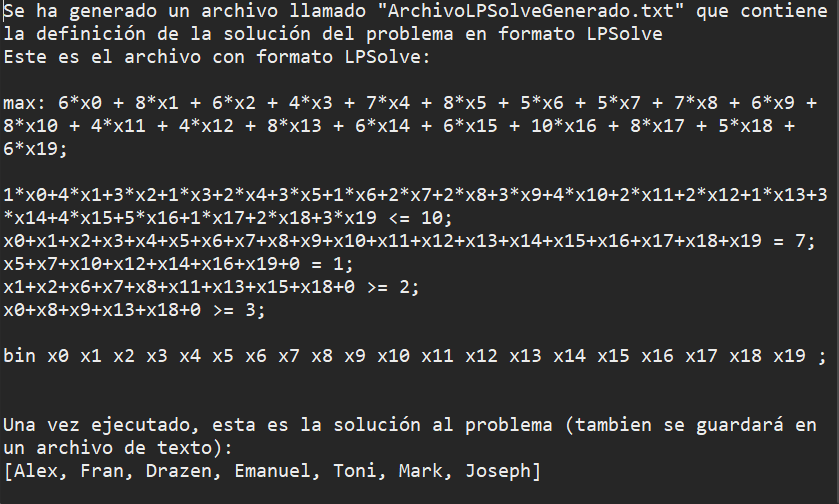
\includegraphics{AlgoritmoPLI.PNG}
  \caption{Volcado de pantalla de la terminal al ejecutar la clase ProblemaBaloncestoPLI}
  \label{fig:pli}
\end{figure}

\begin{figure}[h]
  %TODO: Cambiar
  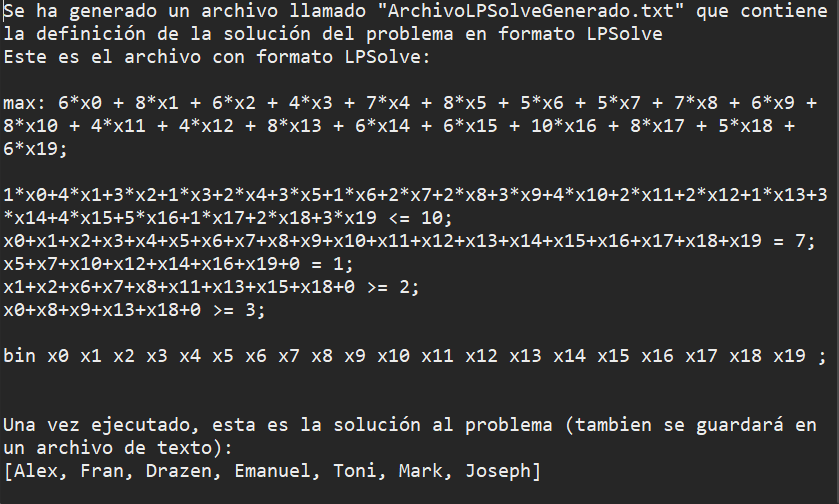
\includegraphics{AlgoritmoPLI.PNG}
  \caption{Volcado de pantalla de la terminal al ejecutar la clase ProblemaBaloncestoAC}
  \label{fig:ag}
\end{figure}

\end{document}
